%----- do not modify this first block,

\documentclass[sigconf,nonacm]{acmart}
\usepackage{tabularx}
\usepackage{natbib}
\usepackage{hyperref}
\usepackage{subfig}
\usepackage{graphicx}
\usepackage{xcolor}


\begin{document}
\title{Which performance indicator is meaningful?}
\author{BART Number 208912}

%% Short summary of the report
\begin{abstract}
	
\end{abstract}

%% builds the first part of the formatted document.
\maketitle

\section{Introduction}
The use of Evolutionary Algorithms (EA) have been popular in solving multi-objective optimisation problems (MOP) due to their population-based approach that enables generation of several elements of the Pareto optimal set in a single run. These are particularly effective in solving complex MOPs with very large spaces, uncertainty, noise, disjoint Pareto curves, etc. Some examples of Multi-objective Evolutionary Algorithms (MOEA) are MOGA, NPGA, NSGA, NSGA-II, PAES, SPEA, SPEA2 and $\epsilon$-MOEA\cite{moea2007, deb2002}. Selecting an efficient MOEA towards solving MOPs of complex nature is crucial to yield accurate optimal points, especially when there is a computational cost attached to it. Performance Indicators (PI) are metrics that are helpful in comparing and ranking multiple MOEAs to determine their efficiencies. There are several PIs that exist in the literature in ranking MOEA. These are broadly divided as per cardinality, convergence, distribution, and both convergence and distribution. Their description is provided in \autoref{sec:Background_PI}. This project explores the correlation between the run time and ranking of two MOEAs using different PIs.

\section{Background}
\subsection{Multi-objective Evolutionary Algorithms}
A multi-objective optimisation problem (MOP) has a number of objective functions which are to be minimised or maximised \cite{deb2001}.\\ A MOP is defined in general form as:
\begin{align*}
	\textbf{Minimize/Maximize} \hspace{0.1cm}
    & f_m(\textbf{x}), \hspace{0.2cm}
    & m = 1, 2, \ldots, M; \\
    \textbf{Subject to} \hspace{0.1cm}
    & g_{j}(\textbf{x}) \ge 0, \hspace{0.2cm}
    & j = 1, 2, \ldots, J; \\
    & h_{k} = 0, \hspace{0.2cm}
    & k = 1, 2, \ldots, K; \\
    & x_{i}^{(L)} \le x_{i} \le x_{i}^{(U)}, \hspace{0.2cm}
    & i = 1, 2, \ldots, n
\end{align*}
A solution \textbf{x} is a vector of \textit{n} decision variables: $\textbf{x} = (x_{1}, x_{2}, \ldots, x_{n})^{T}$. The last set of constraints, $x_{i}^{(L)} \le x_{i} \le x_{i}^{(U)}$, are called variable bounds, restricting each decision variables $x_{i}$ to take a value with a lower $x_{i}^{(L)}$ and an upper $x_{i}^{(U)}$ bound, constituting of the design space $\mathcal{D}$ \cite{deb2002}. "Classical" multi-objective algorithms, such as direct methods and gradient-based methods, are used in solving simple, convex optimisation problems.\\
Deb \cite{deb2002} lists the challenges that "classical" multi-objective algorithms are faced with -
\begin{enumerate}
\item The convergence to an optimal solution depends on the chosen initial solution.
\item Most algorithms tend to get stuck to a suboptimal solution.
\item An algorithm that is efficient in solving one optimisation problem might prove inefficient in solving a different problem.
\item Algorithms are not efficient in handling problems having a discrete search space.
\item Algorithms cannot be efficiently used on a parallel machine.
\end{enumerate}
In such cases, Evolutionary Algorithms prove to be effective in finding optimum solutions to different multi-objective optimisation problems, often simulating complex, real-world design problems. They are advantageous over classical algorithms in the following way \cite{branke2008}:
\begin{enumerate}
\item EAs adopt population-based search, i.e., it generates more than one solution in an iteration. This provides parallel processing power, that helps in achieving a computationally quick overall search. It also finds multiple optimal solutions, thereby facilitating the solution of a multi-modal and multi-objective optimisation problem.
\item EAs adopt a stochastic approach rather than a deterministic approach, yielding to desired outcomes by using biased probability distributions.
\item EAs do not usually use gradient information in their search process. Their approach is more direct, enabling them to be used to a wide variety of optimisation problems.
\end{enumerate}

The two MOEAs considered in this study are NSGA-II and SPEA2.
\subsubsection{NSGA-II}
Non-dominated Sorting Genetic Algorithm
\subsubsection{SPEA2}
\subsection{Performance Indicators} \label{sec:Background_PI}
Performance Indicators for MOEAs are broadly categorised into four aspects \cite{audet2021}:
\begin{enumerate}
\item\textbf{Cardinality:} Cardinality in this context is the number of non-dominated points that are generated by the MOEA.
\item\textbf{Convergence:} This aspect quantifies how close a set of non-dominated points is from the Pareto front.
\item\textbf{Distribution and spread:} This aspect is divided into two sub-groups: First one is how well-distributed the non-dominated points are on the Pareto front; Second one is the extent of Pareto front approximation and whether the Pareto front contains extreme points. This aspect would account for how diverse the non-dominated points are.
\item\textbf{Convergence and distribution:} This aspect considers both the convergence and distribution of the set of non-dominated points.
\end{enumerate}
There are several performance indicators described in the literature by various authors and their application towards MOPs. \\


\section{Methodology and experimental design}
\subsection{Problems used}
There are a range of problems used in this study, extracted from the \textit{jMetalPy} Python module, namely ZDT1, ZDT2, ZDT3, ZDT4, ZDT6, DTLZ1, DTLZ2, DTLZ3, DTLZ4, DTLZ5, DTLZ6, and DTLZ7, to perform analysis. These problem types are diverse in nature, and their characteristics are tabulated below.\\
\begin{table*}[t]
\centering
\begin{tabular}{|c|c|c|c|}
\hline
Problem type & Number of objectives & Number of variables & Problem description \\
\hline
ZDT1 & 2 & 30 & Continuous, unconstrained, convex pareto front \\
ZDT2 & 2 & 30 & Continuous, unconstrained, non-convex pareto front \\
ZDT3 & 2 & 30 & Continuous, unconstrained, disconnected pareto front \\
ZDT4 & 2 & 30 & Continuous, unconstrained, convex pareto front \\
ZDT6 & 2 & 30 & Non-uniform, unconstrained, non-convex pareto front \\
\hline
\end{tabular}
\caption{Description of problems considered}
\end{table*}
\subsection{MOEAs used}
The two MOEAs used for analysis is Non-dominated Sorting Genetic Algorithm (NSGA-II) and Strength Pareto Evolutionary Algorithm 2 (SPEA2). Their characteristics were described in section 2. The NSGA-II and SPEA2 methods are pre-defined in the \textit{jMetalPy} Python module, and were utilised with the following arguments to perform analysis.
\subsection{Performance Indicators}
The three performance indicators used for analysis are IGD (convergence-focussed), $\Delta$-metric (diversity- and distribution-focussed), and hypervolume indicator (convergence- and distribution-focussed).
\subsubsection{IGD}
Pymoo contains a pre-defined function to calculate IGD with respect to the true Pareto front, and outputs the measure when compared to each of the algorithm-generated set of solutions in the form of their respective Pareto fronts.
\subsubsection{$\Delta$-metric}
The $\Delta$-metric is not defined in any of the MOP libraries present in Python, so this was defined as:


\section{Analysis and results}
\begin{figure*}
\begin{tabular}{cccc}
\centering
\subfloat[ZDT1:4000]{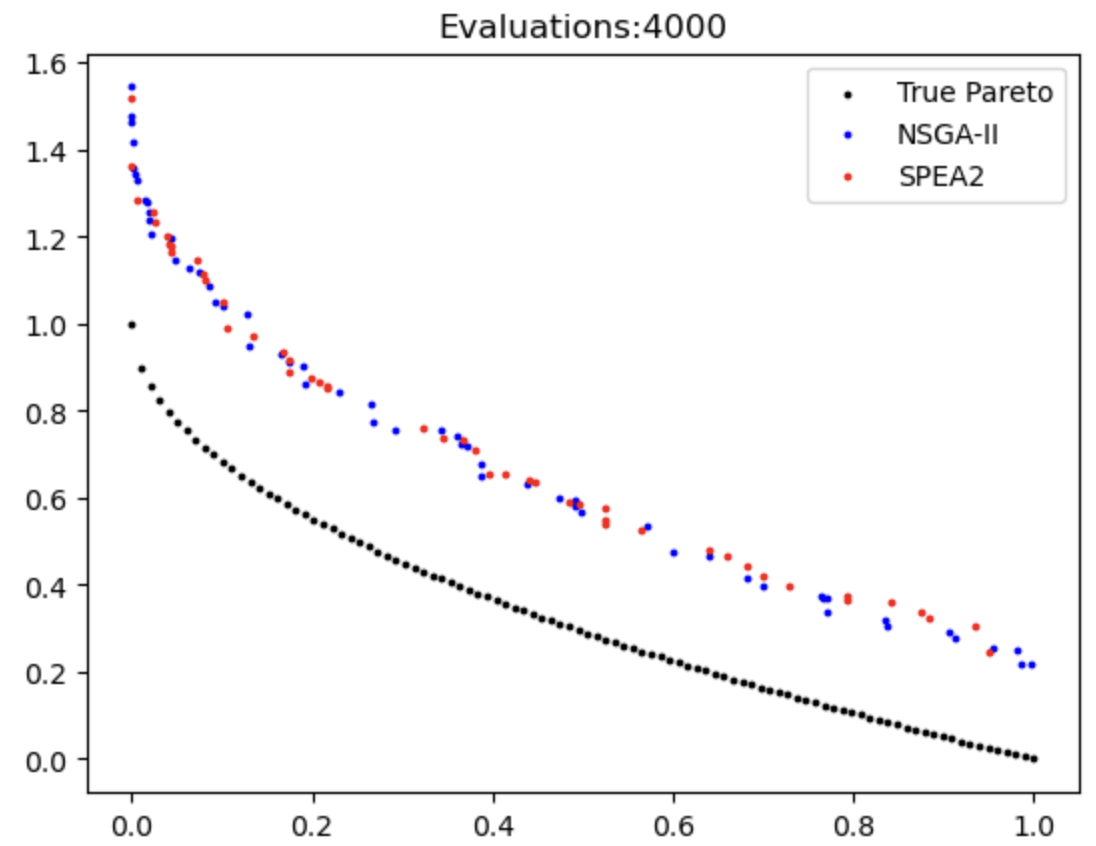
\includegraphics[width = 1.5in]{ZDT1_4e3.png}} &
\subfloat[ZDT1:8000]{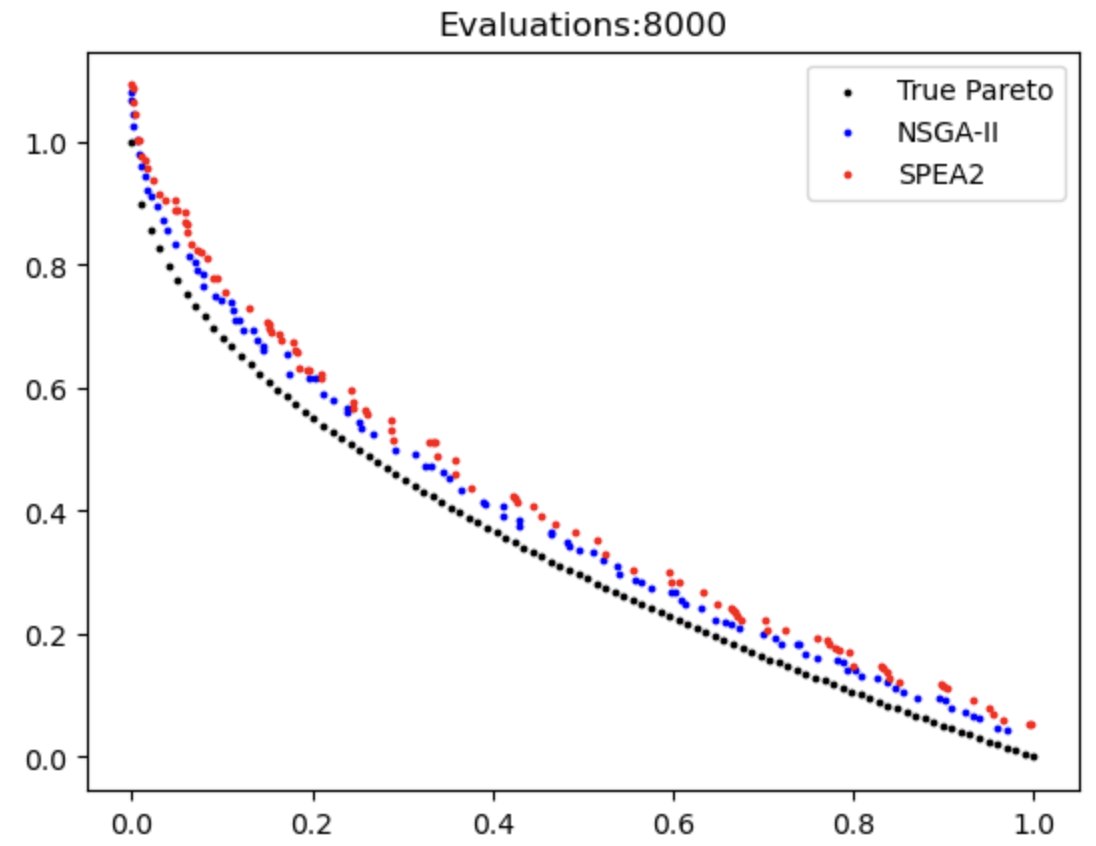
\includegraphics[width = 1.5in]{ZDT1_8e3.png}} &
\subfloat[ZDT1:12000]{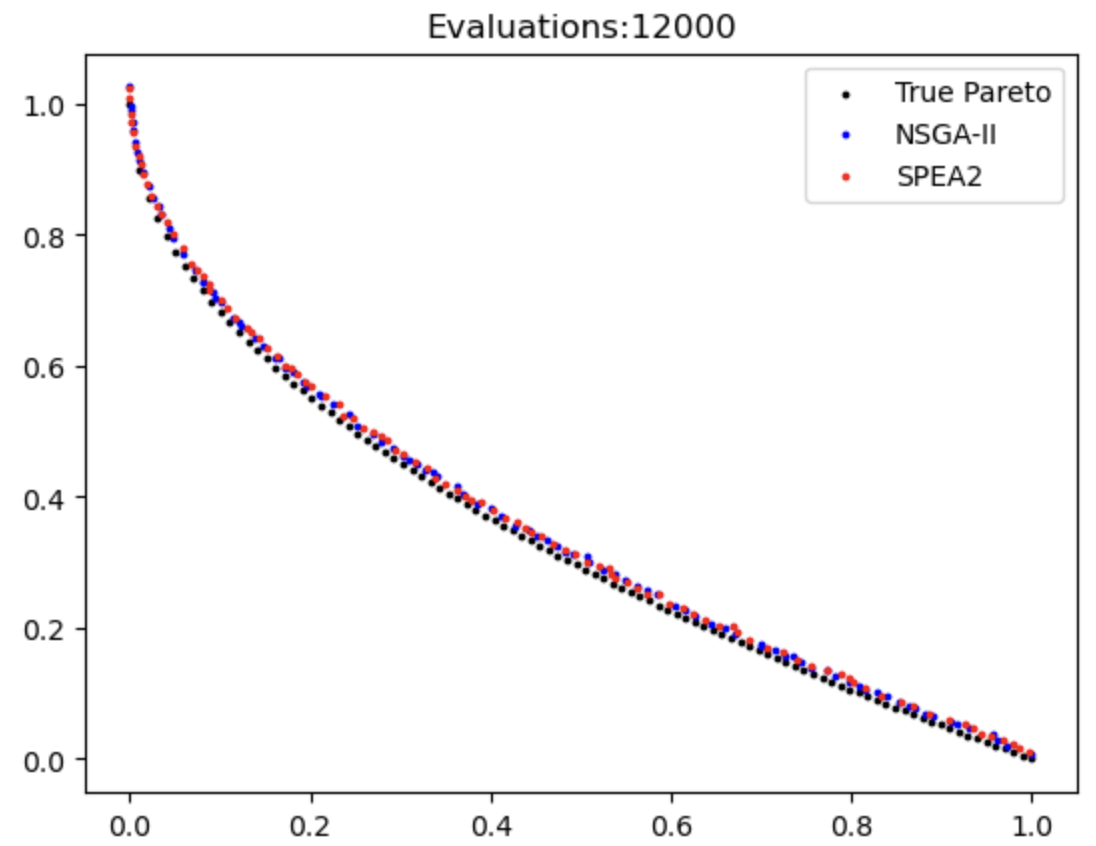
\includegraphics[width = 1.5in]{ZDT1_12e3.png}} &
\subfloat[ZDT1:16000]{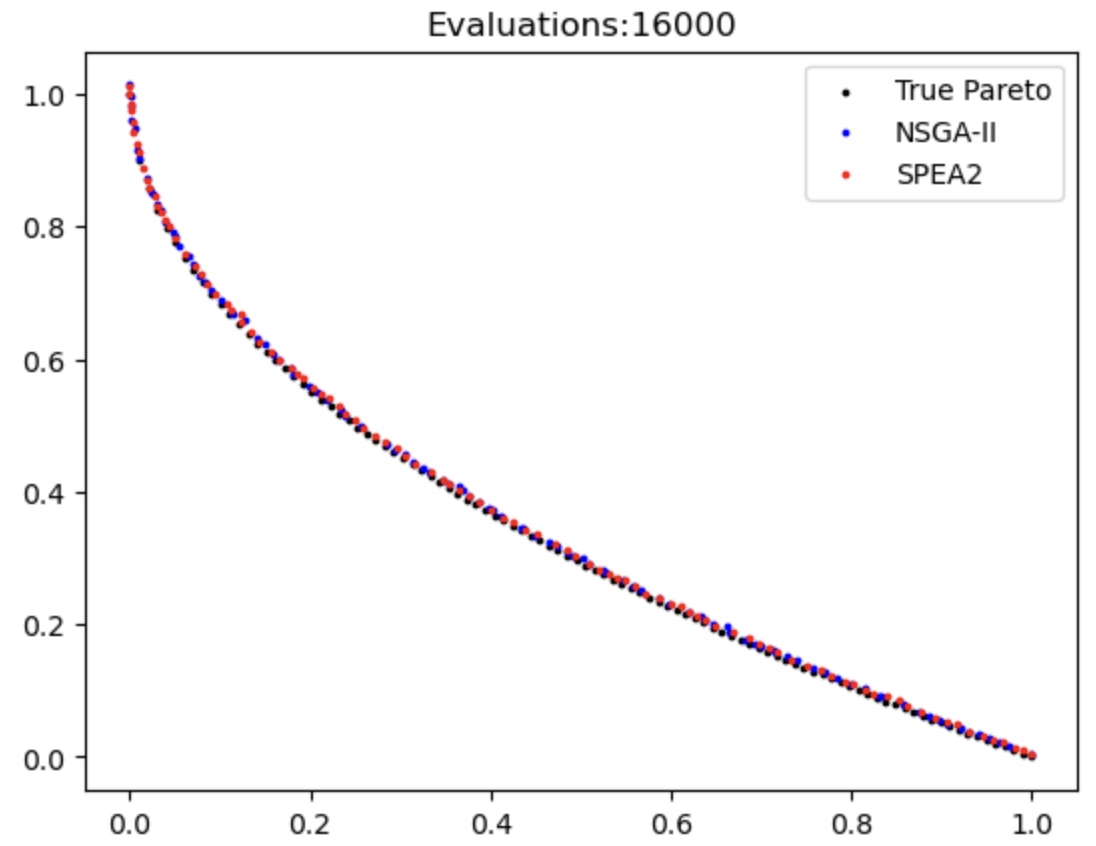
\includegraphics[width = 1.5in]{ZDT1_16e3.png}}\\
\subfloat[ZDT2:4000]{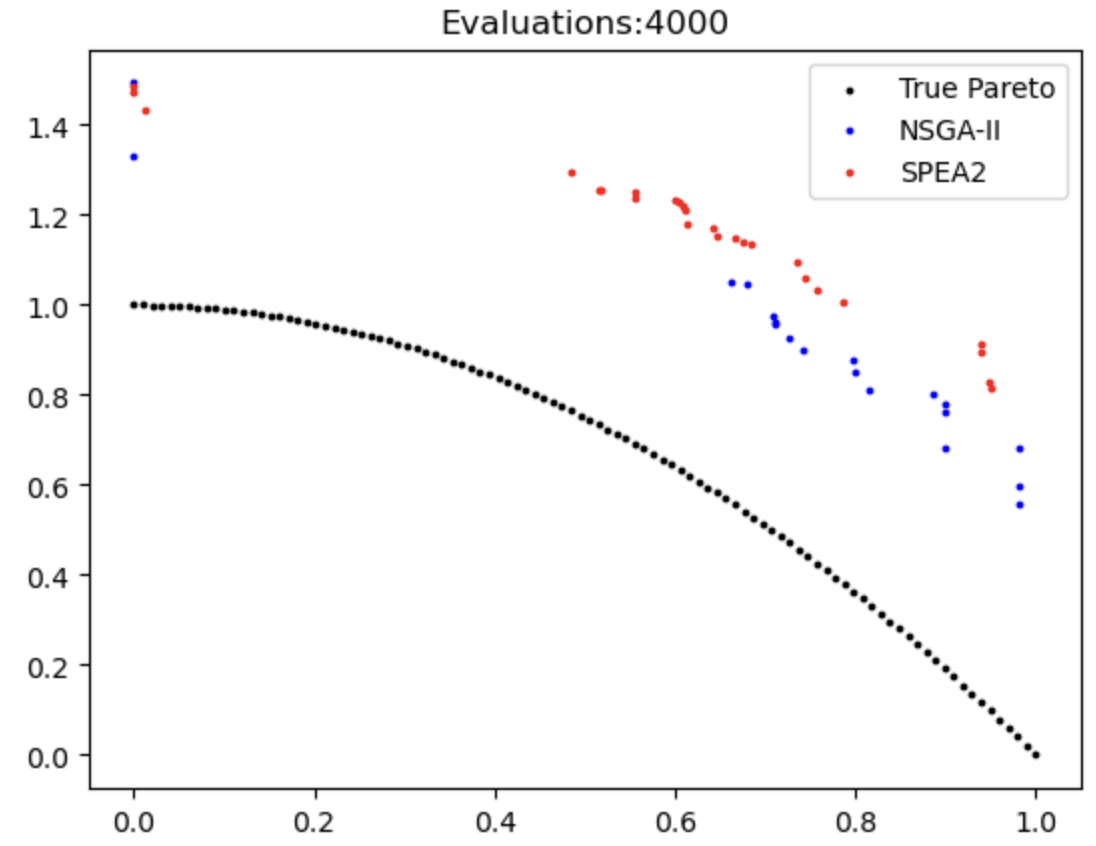
\includegraphics[width = 1.5in]{ZDT2_4e3.png}} &
\subfloat[ZDT2:8000]{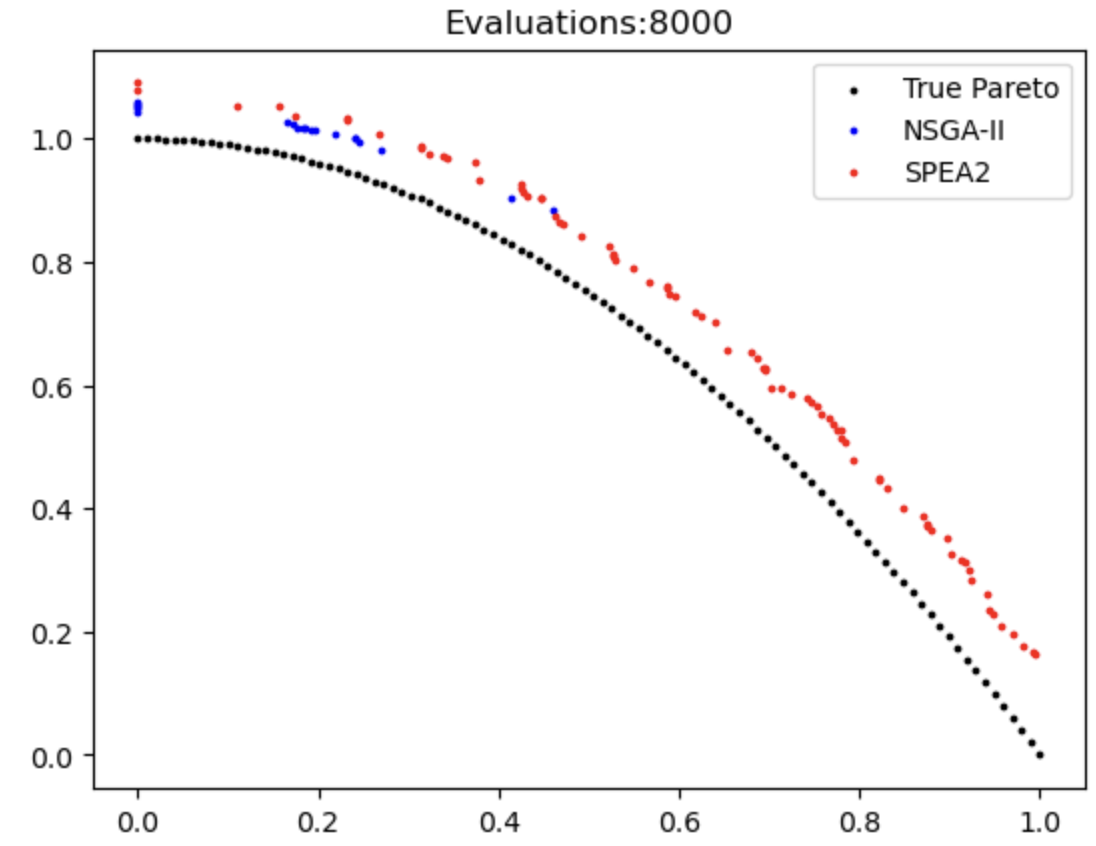
\includegraphics[width = 1.5in]{ZDT2_8e3.png}} &
\subfloat[ZDT2:12000]{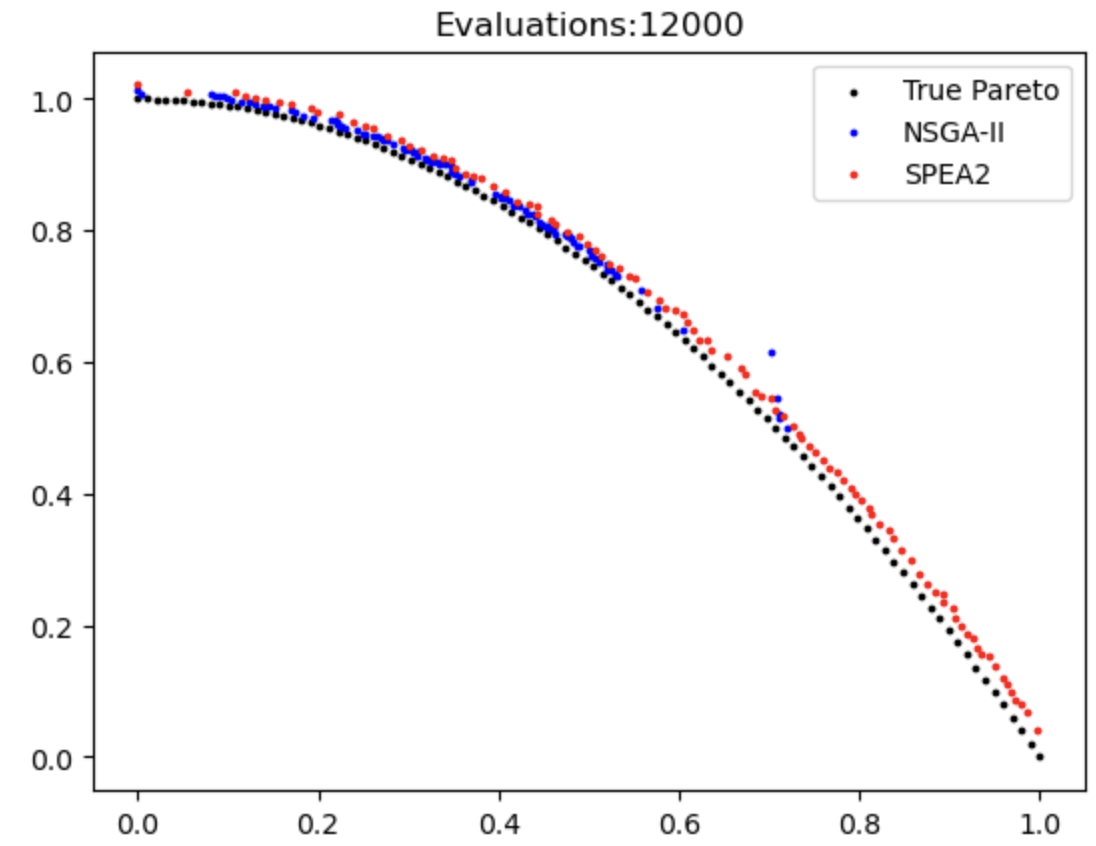
\includegraphics[width = 1.5in]{ZDT2_12e3.png}} &
\subfloat[ZDT2:16000]{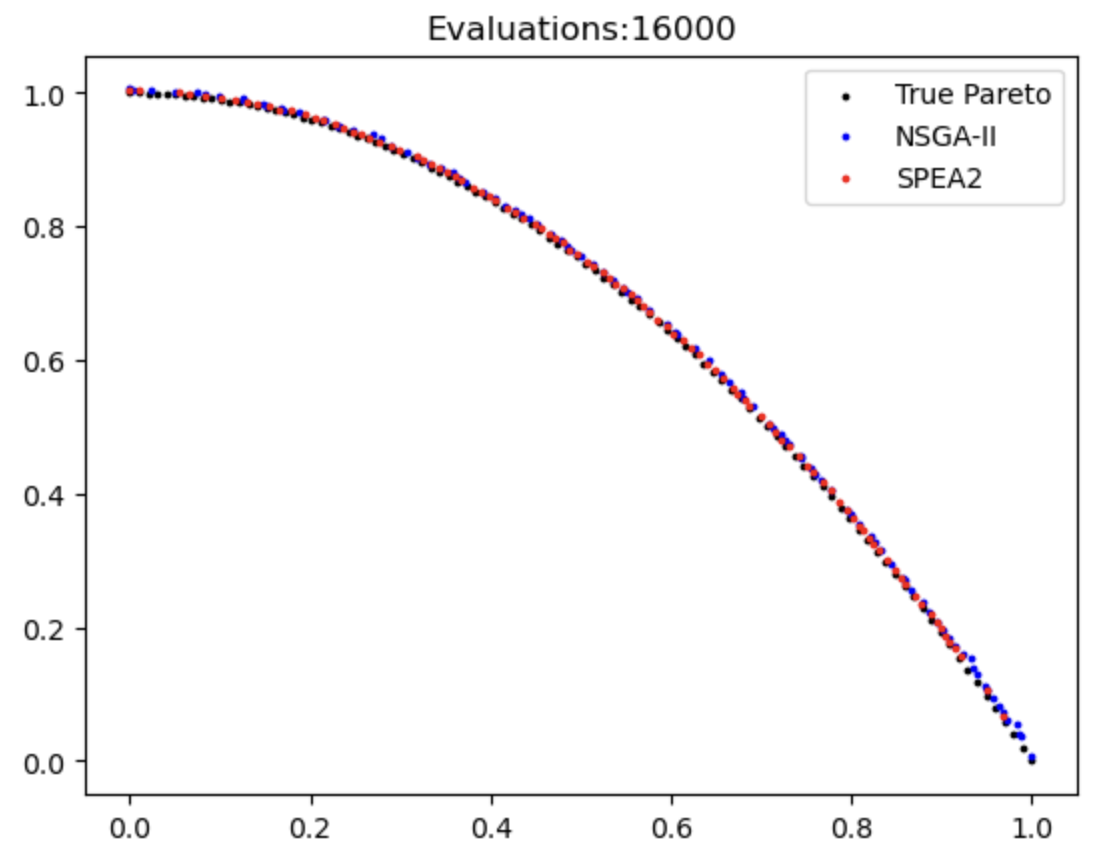
\includegraphics[width = 1.5in]{ZDT2_16e3.png}}\\
\subfloat[ZDT3:4000]{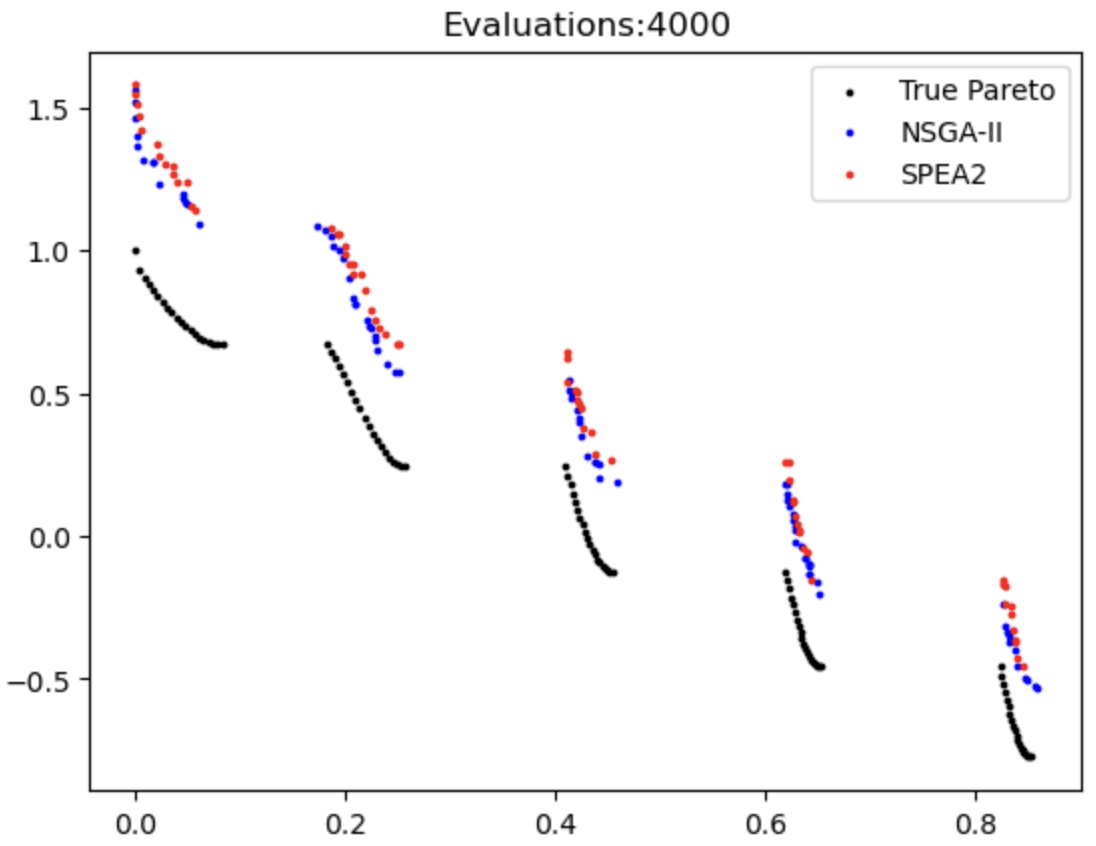
\includegraphics[width = 1.5in]{ZDT3_4e3.png}} &
\subfloat[ZDT3:8000]{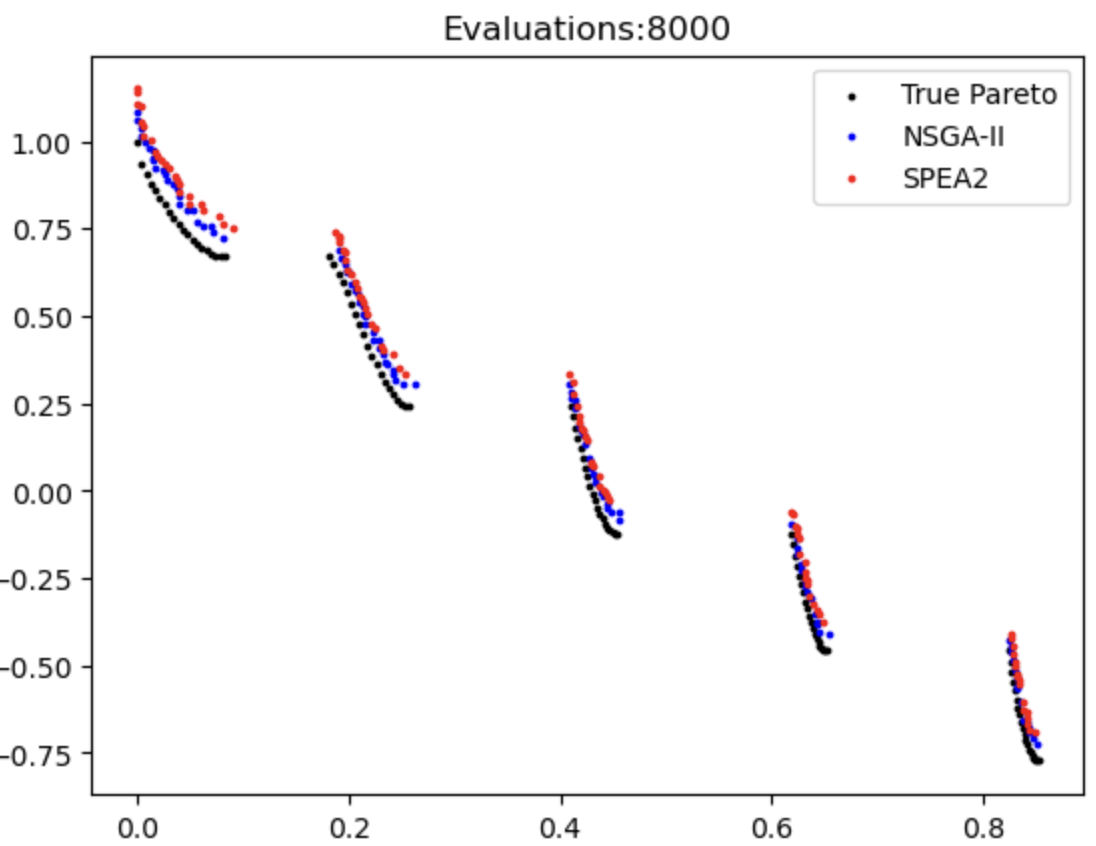
\includegraphics[width = 1.5in]{ZDT3_8e3.png}} &
\subfloat[ZDT3:12000]{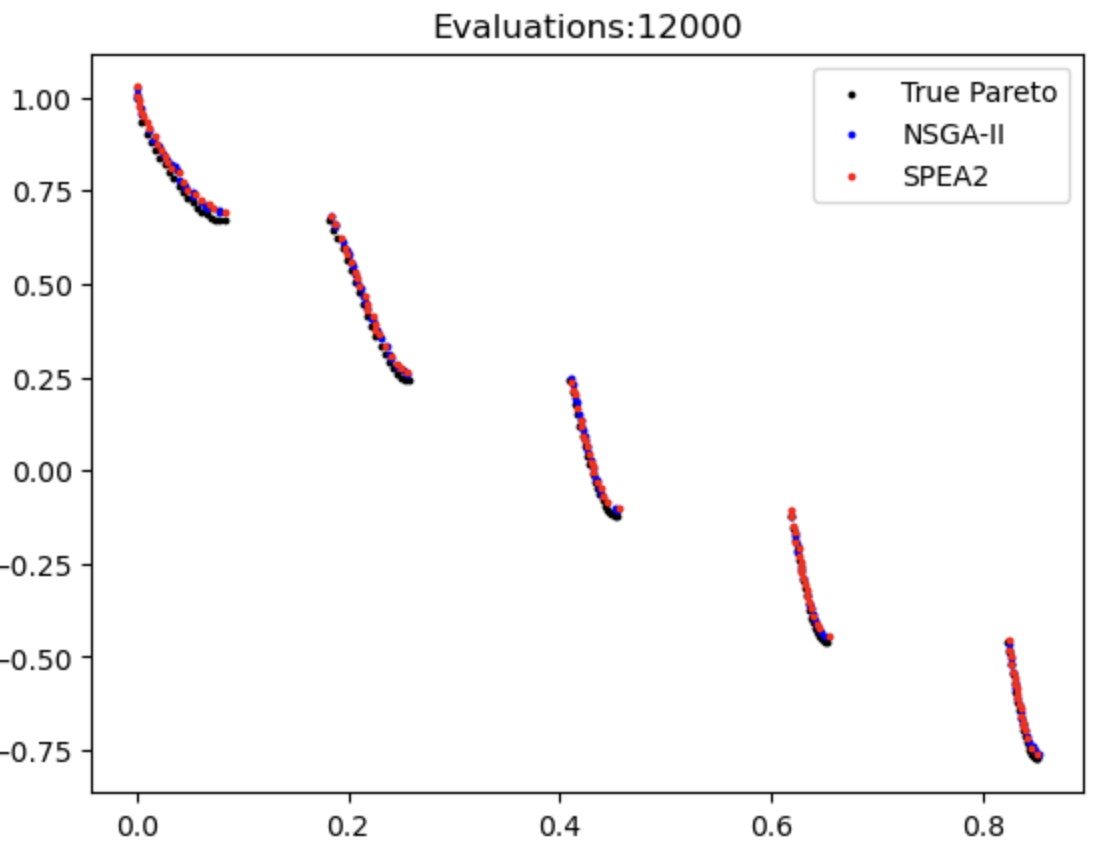
\includegraphics[width = 1.5in]{ZDT3_12e3.png}} &
\subfloat[ZDT3:16000]{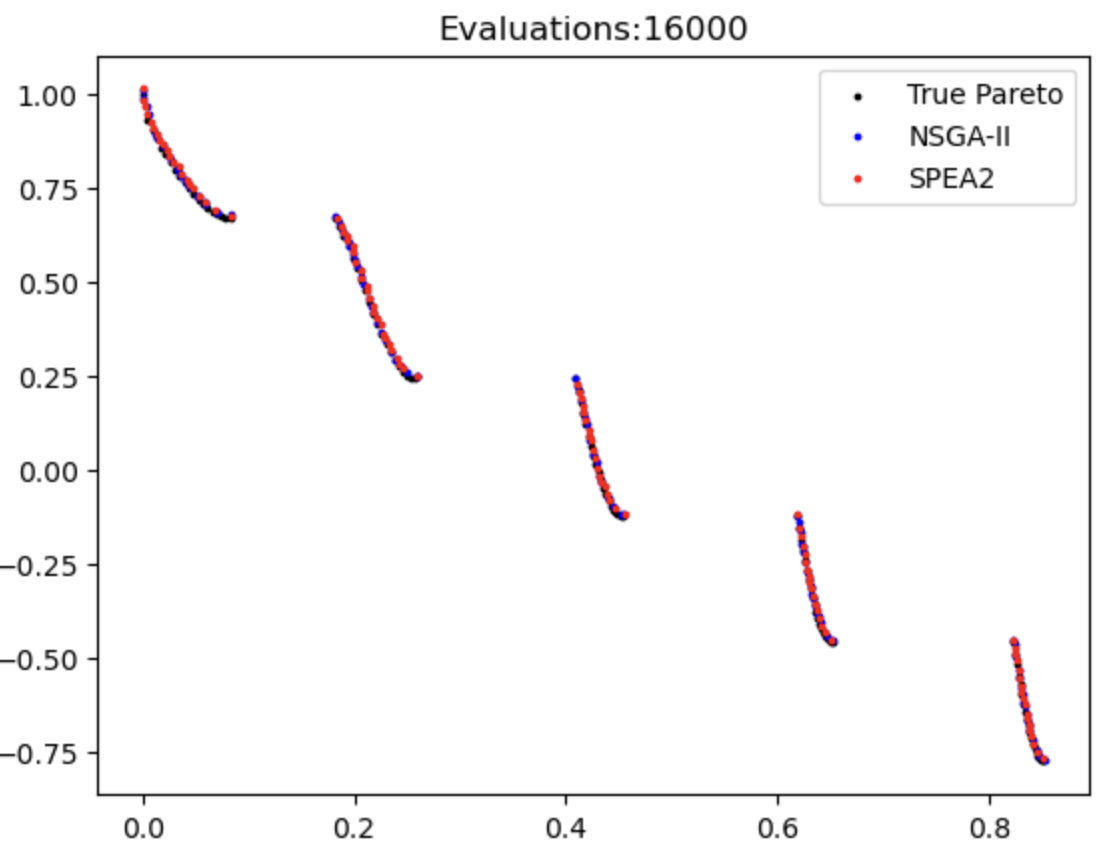
\includegraphics[width = 1.5in]{ZDT3_16e3.png}}\\
\subfloat[ZDT4:4000]{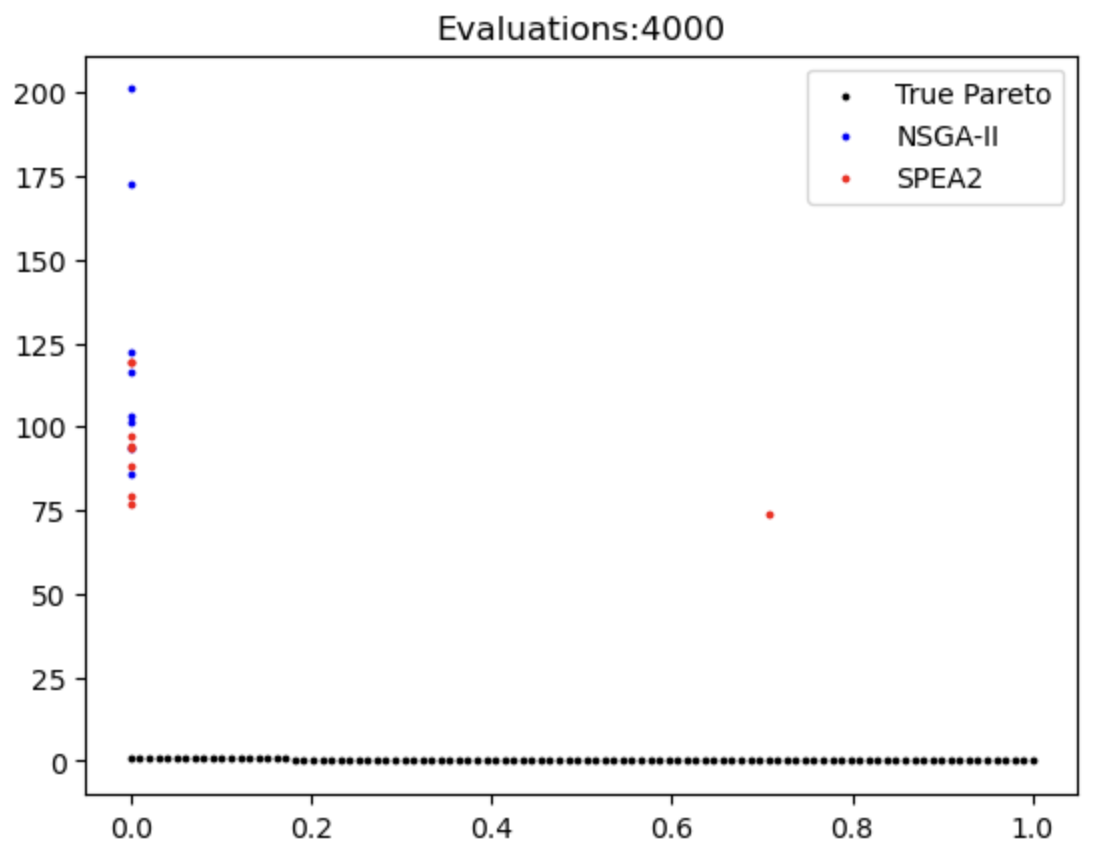
\includegraphics[width = 1.5in]{ZDT4_4e3.png}} &
\subfloat[ZDT4:28000]{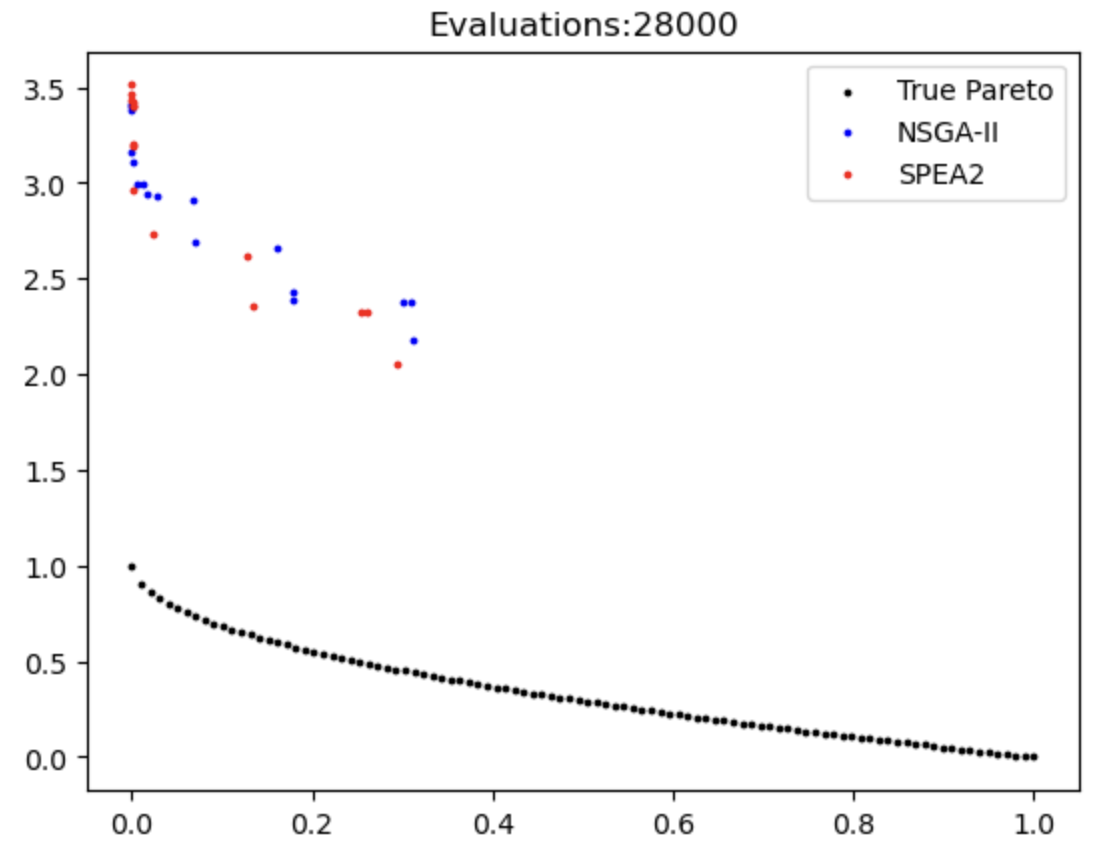
\includegraphics[width = 1.5in]{ZDT4_28e3.png}} &
\subfloat[ZDT4:54000]{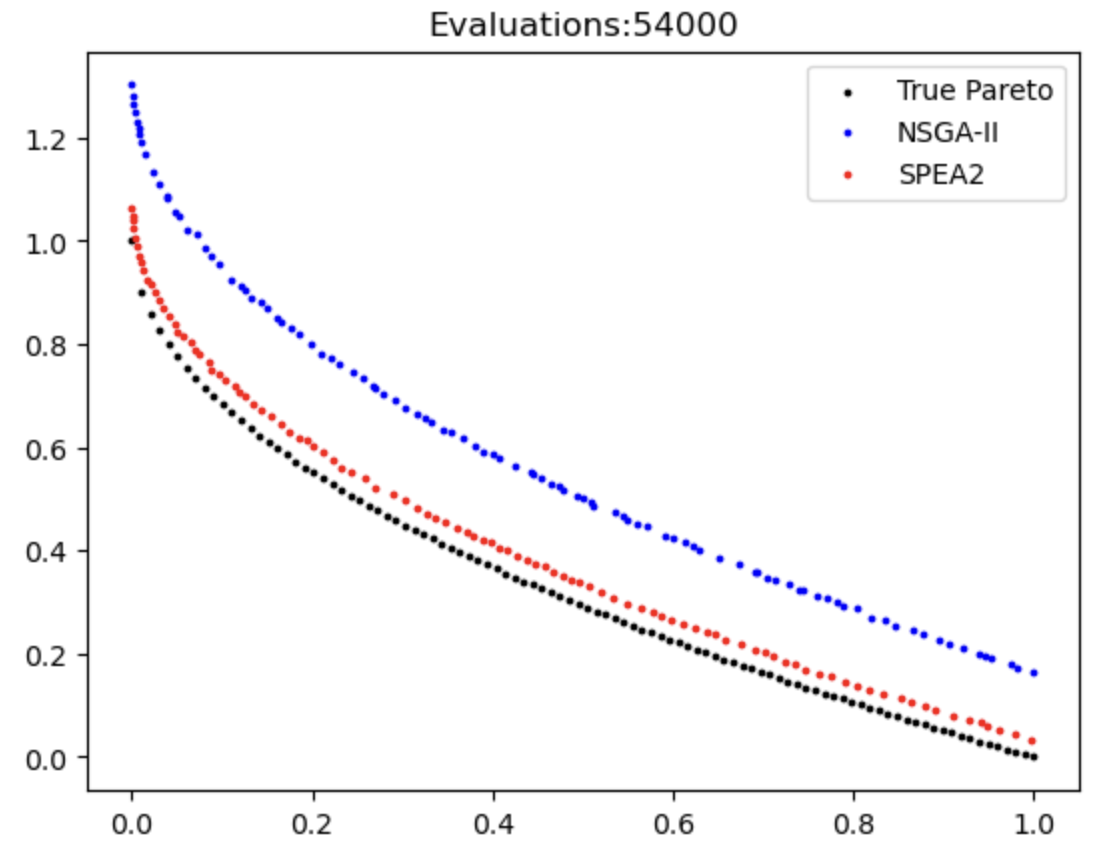
\includegraphics[width = 1.5in]{ZDT4_54e3.png}} &
\subfloat[ZDT4:72000]{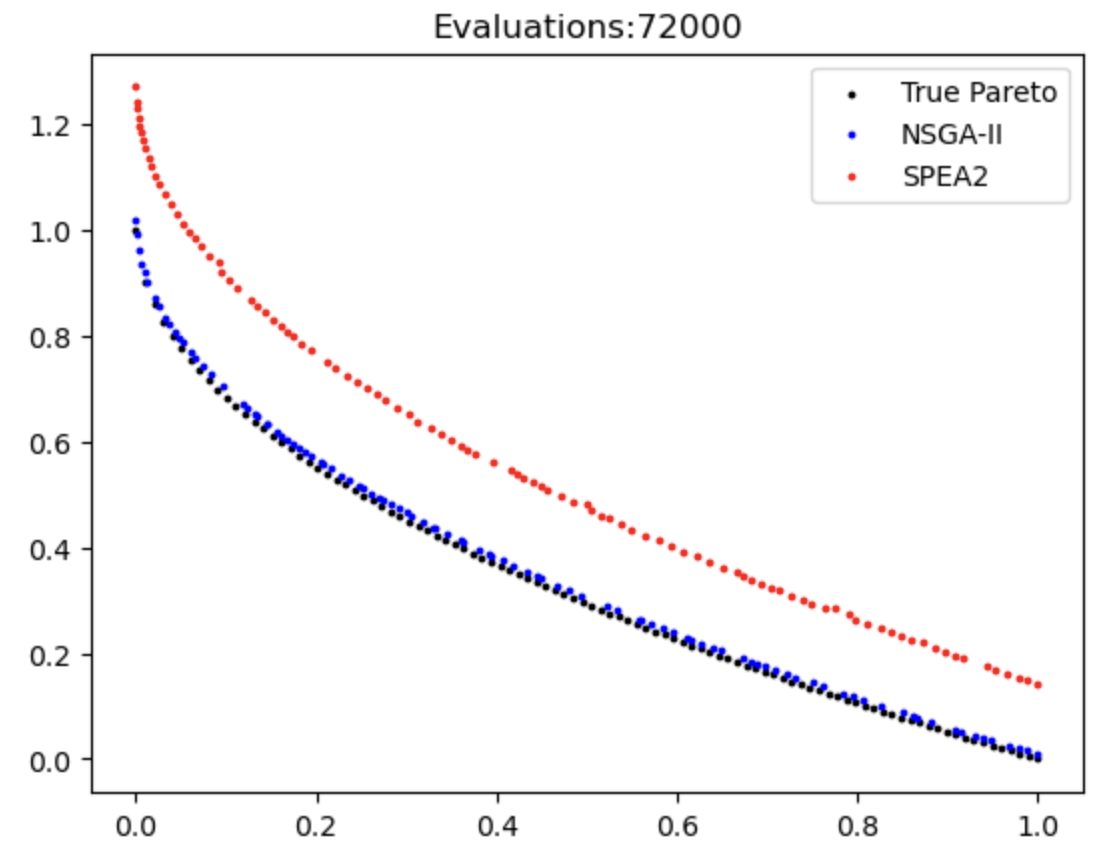
\includegraphics[width = 1.5in]{ZDT4_72e3.png}}\\
\subfloat[ZDT6:4000]{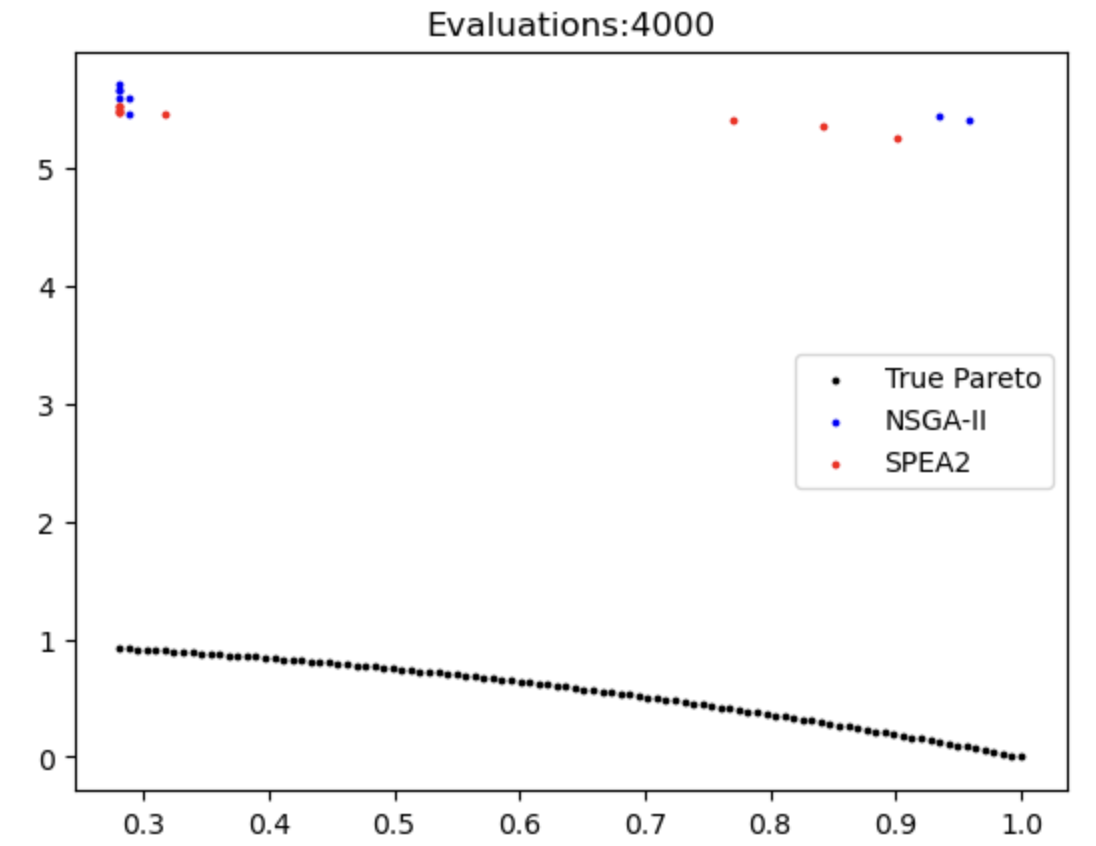
\includegraphics[width = 1.5in]{ZDT6_4e3.png}} &
\subfloat[ZDT6:28000]{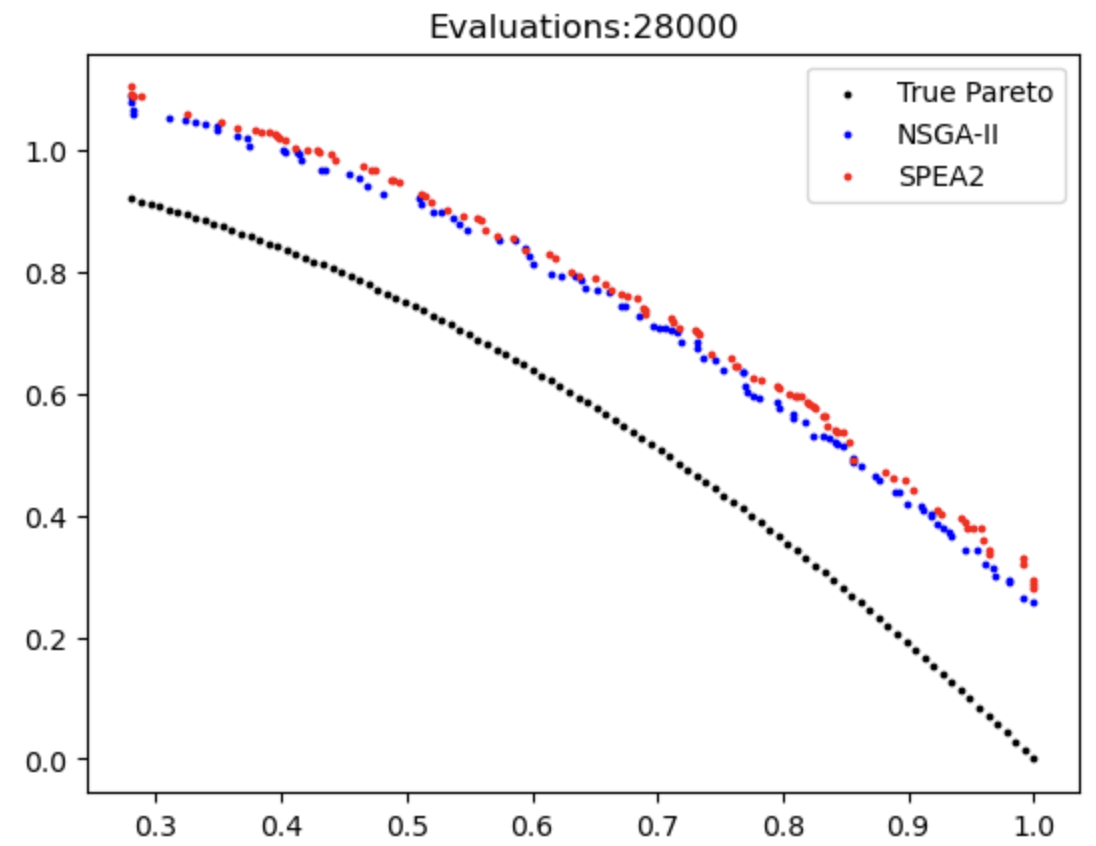
\includegraphics[width = 1.5in]{ZDT6_28e3.png}} &
\subfloat[ZDT6:54000]{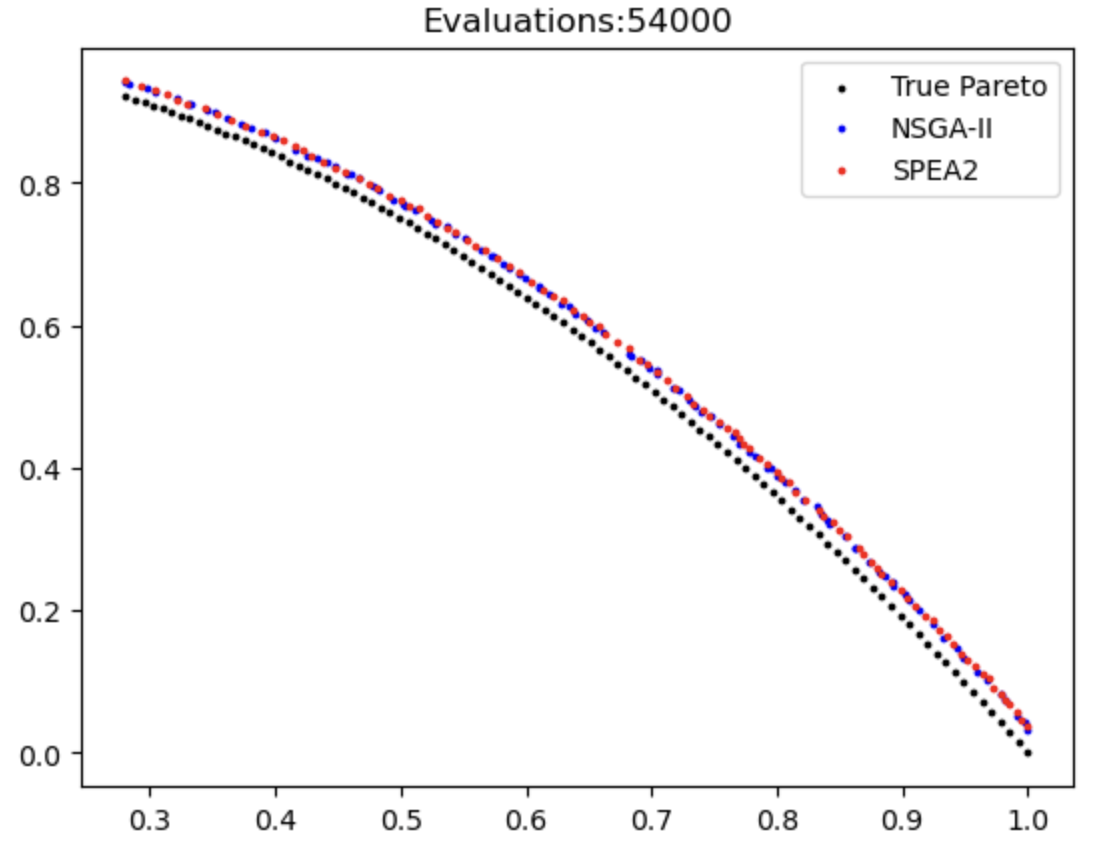
\includegraphics[width = 1.5in]{ZDT6_54e3.png}} &
\subfloat[ZDT6:72000]{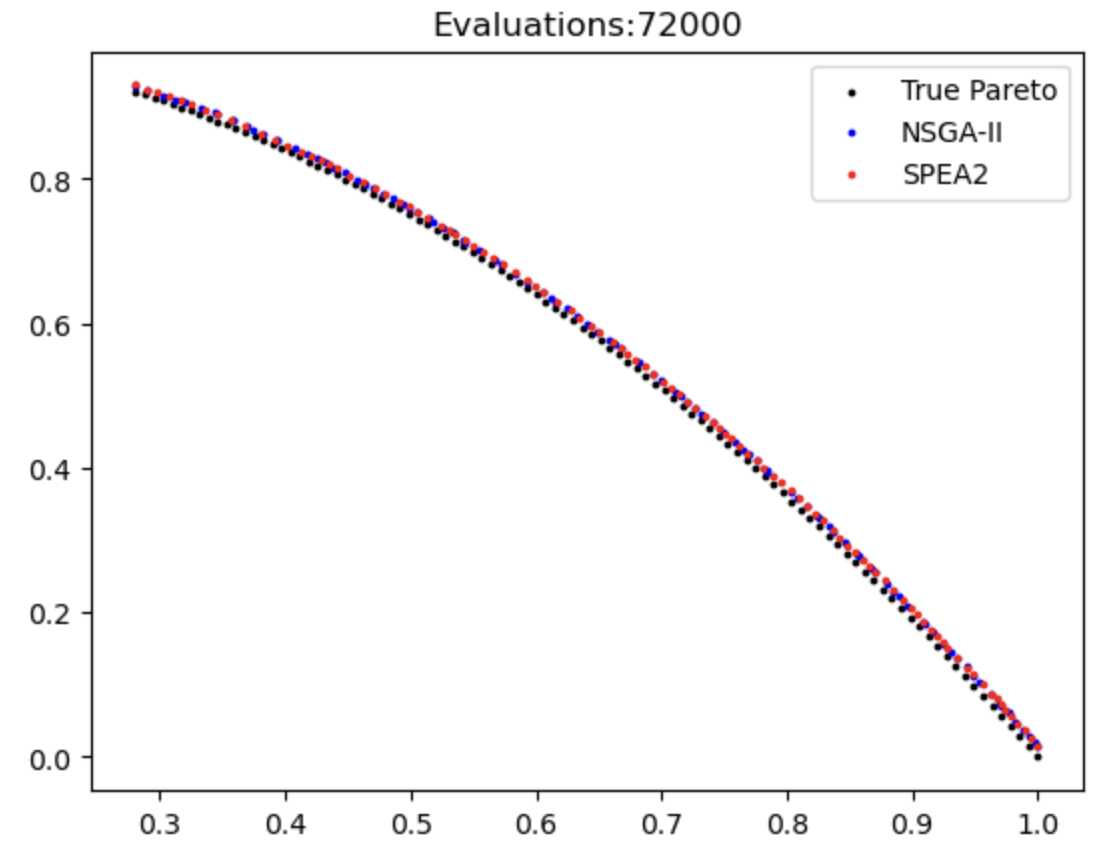
\includegraphics[width = 1.5in]{ZDT6_72e3.png}}
\end{tabular}
\caption{For the above simulations, the problem name and number of evaluations are given as graph titles. The \underline{\textcolor{blue}{blue}} points represent set of solutions for NSGA-II, and the \underline{\textcolor{red}{red}} points represent set of solutions for SPEA2, while the \underline{black} points represent the true Pareto front}
\end{figure*}


\section{Discussion and future work}

\bibliographystyle{ACM-Reference-Format}
\bibliography{references.bib} 



\end{document}
